\section{Regressão Linear}

\begin{frame}{Regressão Linear}
  \begin{block}{Problema:}
    \begin{itemize}
      \item Dados $n$ inputs e $n$ outputs, $(x,y)$, aproximar $f(x) = y$.
      \item Encontrar $w_0$, $w_1$ de forma que o erro em $\hat{f}(x) = w_1 x + w_0$ seja aceitável.
    \end{itemize}
  \end{block}

  \begin{figure}[t]
    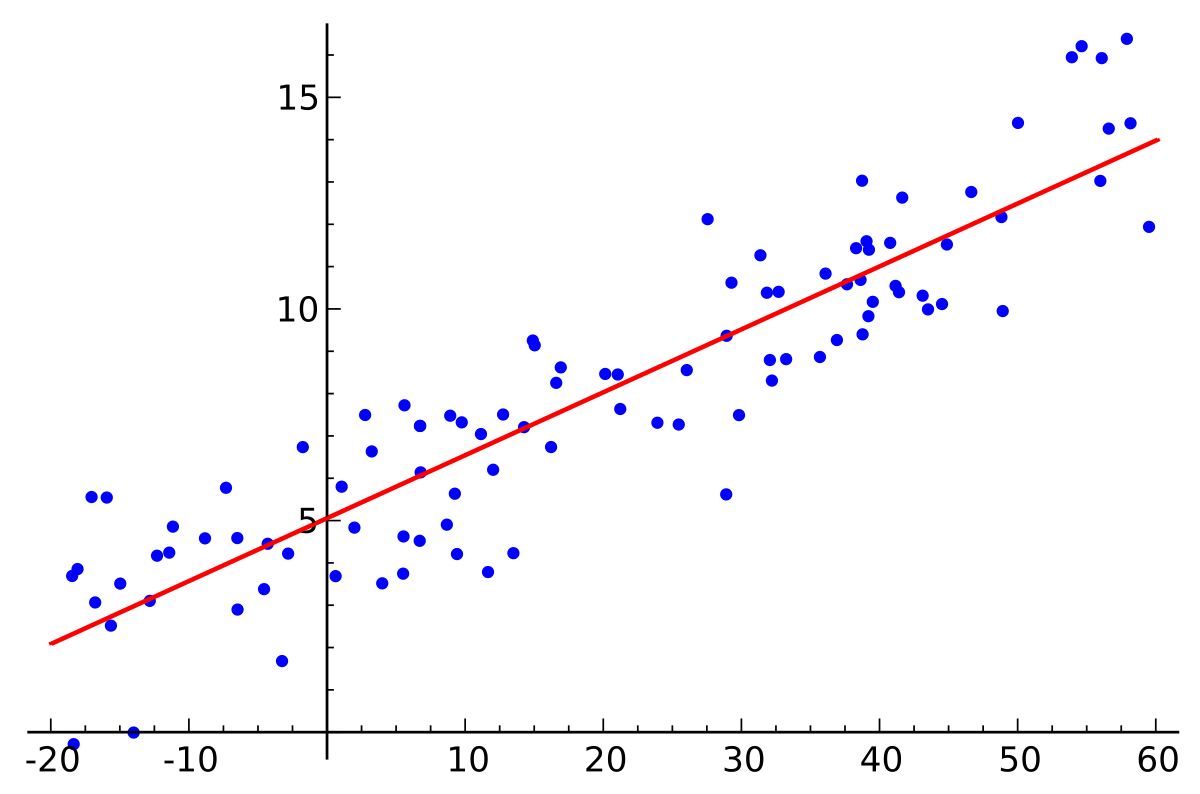
\includegraphics[width=0.5\textwidth]{lr.png}
    \centering
  \end{figure}

\end{frame}

\begin{frame}{Regressão Linear}
  \[ E(w_0, w_1 \mid x) = \frac{1}{2} \sum_{i=1}^{n} \left[y_i - (w_1 x_i + w_0)^2 \right] \]

  Para encontrar $w_0$ e $w_1$ que minizam $E$:

  \[ \frac{\partial E}{\partial w_0} = 0 \qquad \frac{\partial E}{\partial w_1} = 0 \]

  Simplificando:

  \begin{align*}
    \sum_{i=1}^{n} y_i &= n w_0 + w_1 \sum_{i=1}^{n} x_i\\
    \sum_{i=1}^{n} y_i x_i &= w_0 \sum_{i=1}^{n} x_i + w_1 \sum_{i=1}^{n} x_i^2
  \end{align*}
\end{frame}

\begin{frame}{Regressão Linear}

  \begin{align*}
    \sum_{i=1}^{n} y_i &= n w_0 + w_1 \sum_{i=1}^{n} x_i\\
    \sum_{i=1}^{n} y_i x_i &= w_0 \sum_{i=1}^{n} x_i + w_1 \sum_{i=1}^{n} x_i^2
  \end{align*}

  \begin{align*}
    A &= \begin{bmatrix}
      n & \sum x_i \\
      \sum x_i & \sum x_i^2
    \end{bmatrix} \qquad \vt{b} = \begin{bmatrix} w_0 \\ w_1 \end{bmatrix} \\
    \vt{y} &= \begin{bmatrix} \sum y_i \\ \sum y_i x_i \end{bmatrix} \quad A \vt{w} = y
  \end{align*}

  Ou seja, $ \vt{w} = A^{-1} \vt {y} $.
\end{frame}

